\documentclass[UTF8, fontset=none,12pt]{ctexart}
\usepackage{xeCJK}
\usepackage{titlesec} 
\usepackage{hyperref}
\usepackage{graphicx}
\usepackage{subcaption}
\usepackage{setspace}
\usepackage[a4paper, margin=2.45cm]{geometry}
% 標楷體
\setCJKmainfont[AutoFakeBold=3, AutoFakeSlant=.2]{DFKai-SB}
% \titleformat{章節層級}[形狀]{字體設定}{標號}{標號與標題間距}{標題前指令}
% \fontsize{字號}{行距}
\titleformat{\section}{\fontsize{18}{22}\bfseries}{\thesection}{1em}{}
\titlespacing{\section}{0pt}{1.5ex plus .1ex minus .2ex}{1pc}
\titleformat{\subsection}{\fontsize{14}{17}\bfseries}{\thesubsection}{1em}{}
\title{\fontsize{25}{30}\selectfont 地科探究：聖嬰年\&反聖嬰年的7月台灣海峽海溫、黑潮強度以及氣溫差異}
\author{\fontsize{16}{14}\selectfont 羅東高中\hspace{4cm}賴洧霖}
\renewcommand{\figurename}{圖}
\begin{document}
\pagestyle{plain}%page number and header
\date{}
\maketitle
\section{摘要}%newpage use \newpage to start a new page
我們針對聖嬰現象與反聖嬰現象對台灣西海域的影響進行了深入研究。
通過分析歷史數據和模擬結果，最終發現聖嬰現象會導致台灣西半部海域的水溫升高。
而反聖嬰現象則會導致水溫下降。至於氣溫方面，聖嬰年各地的溫度明顯較平均高出許多，
而反聖嬰雖也升溫但整體升溫幅度並不高。年平均溫則較低。\\

{\fontsize{16}{19}\selectfont
 本研究以代表性年份進行初步比較：2016年為聖嬰年，2021年為反聖嬰年。
 }
\section{關鍵字}
地球科學、聖嬰現象、反聖嬰現象、台灣西半部海域水溫變化、氣溫變化、NOAA數據分析
 \href{https://weilinlai719.github.io/earth-science-explore/}
 {聖嬰現象與反聖嬰現象觀察}
\section{簡介}
這是一份關於聖嬰年與反聖嬰年對台灣海峽海溫、黑潮強度以及氣溫差異的研究報告。
我們將通過分析NOAA的數據庫中的歷史數據來探討這些現象對台灣西半部海域的影響。

在選擇題目時，我們想到NOAA的資料庫中有關聖嬰現象和反聖嬰現象的數據。
這些現象對全球氣候有著重要的影響，特別是對台灣西半部海域的水溫變化。
因此，我們決定以這個主題作為我們的研究對象。
\newpage
\section{研究目的}
本研究旨在探討聖嬰現象和反聖嬰現象對台灣西半部海域水溫以及台灣整體氣溫的影響。
通過分析歷史數據和模擬結果，我們希望能夠更好地理解這些現象對台灣氣候的影響，
並為未來的氣候預測提供參考。
\section{研究方法}
本報告採用NOAA的數據庫中的歷史數據進行分析，
以此評估聖嬰現象和反聖嬰現象對台灣西半部海域水溫的影響，
以及對黑潮強度和氣溫的影響。
並進行圖表製作以展示水溫變化。
處理方式（平均、距平）

\section{結果與討論}
通過分析歷史數據，我們發現聖嬰現象會導致台灣西半部海域的水溫升高，
而反聖嬰現象則會導致水溫下降。
    \begin{figure}[h]
    \centering
    \begin{subfigure}[b]{0.45\textwidth}
        \centering
        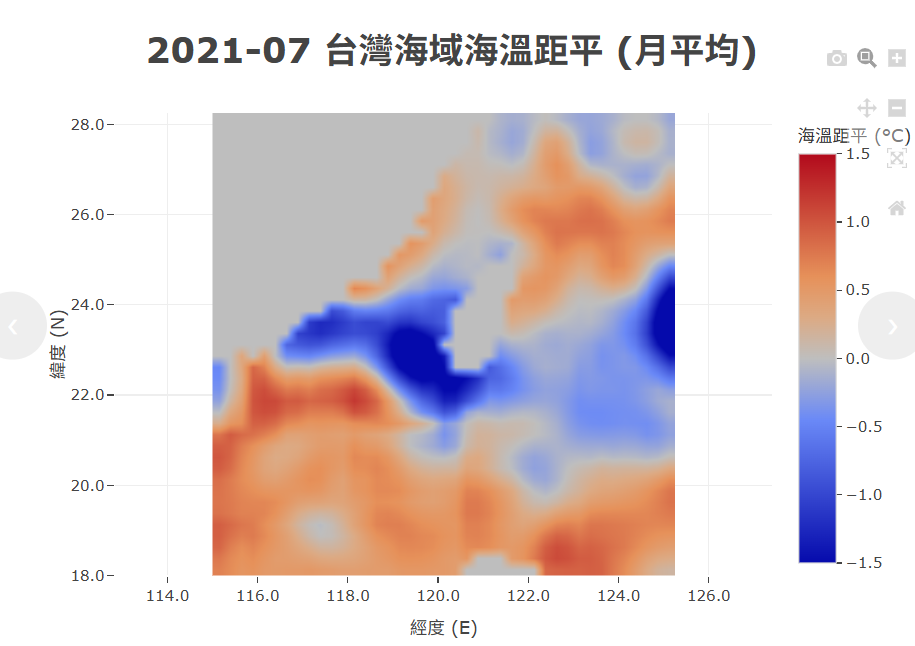
\includegraphics[width=\textwidth]{2021-7.png}
        \caption{2021年7月的水溫分布圖(反聖嬰現象)}
    \end{subfigure}
    \hfill % 把兩張圖推向左右兩端
    \begin{subfigure}[b]{0.45\textwidth}
        \centering
        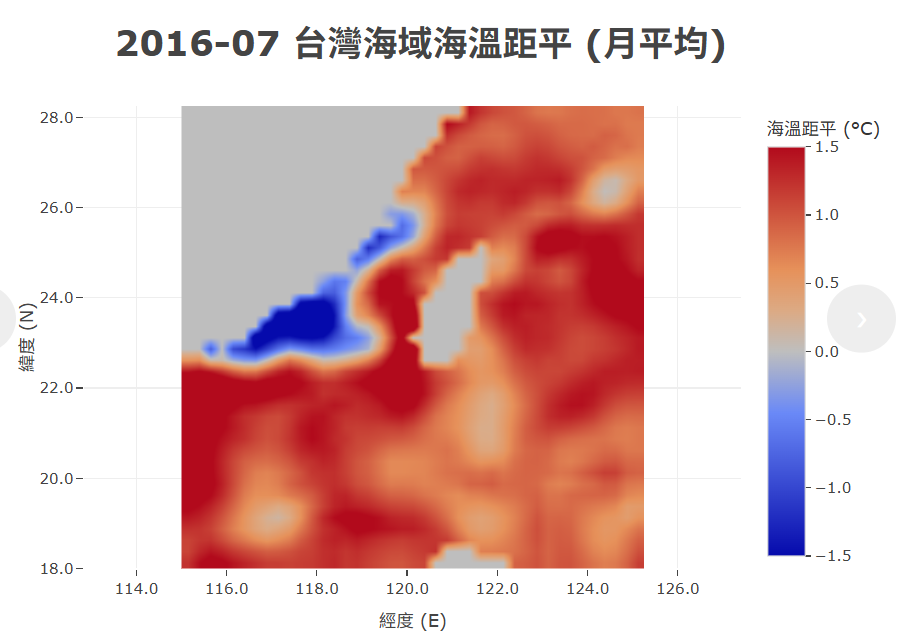
\includegraphics[width=\textwidth]{2016-7.png}
        \caption{2016年7月的水溫分布圖(聖嬰現象)}
    \end{subfigure}
    
    \caption{聖嬰與反聖嬰現象對水溫的影響}
    \label{fig:two_images}
    \end{figure}

\noindent 聖嬰年時，海峽溫度明顯較高，氣溫明顯較高，推測黑潮強度增加；\\
反聖嬰年時，海峽溫度明顯較低，氣溫明顯較低，推測黑潮強度減弱。\\
     \begin{figure}[h]
    \centering
    \begin{subfigure}[b]{0.45\textwidth}
        \centering
        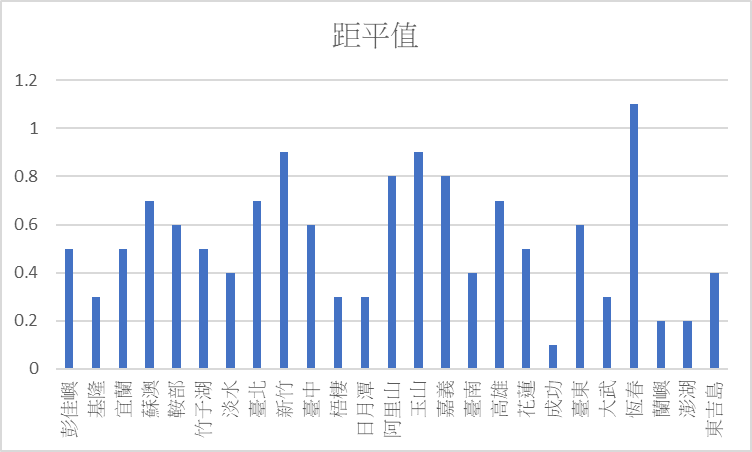
\includegraphics[width=\textwidth]{2016-tem.png}
        \caption{2016年7月氣溫距平值}
    \end{subfigure}
    \hfill % 把兩張圖推向左右兩端
    \begin{subfigure}[b]{0.45\textwidth}
        \centering
        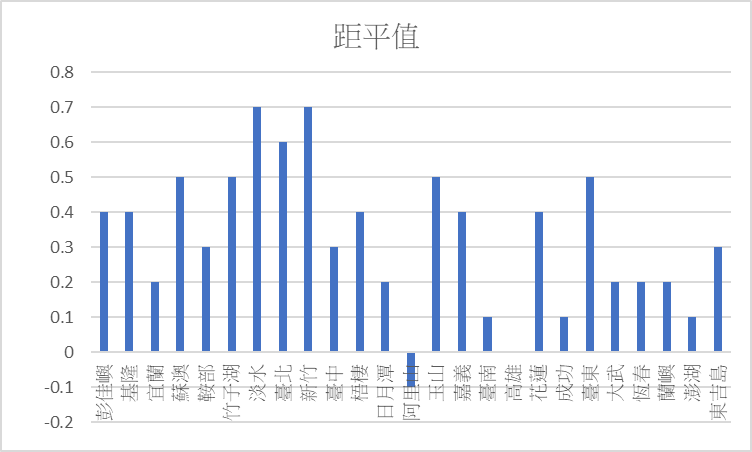
\includegraphics[width=\textwidth]{2021-tem.png}
        \caption{2021年7月氣溫距平值}
    \end{subfigure}
    \caption{聖嬰與反聖嬰現象對台灣氣溫距平的影響}
    \label{fig:two_tables}
    \end{figure}

    \begin{figure}
    \centering
    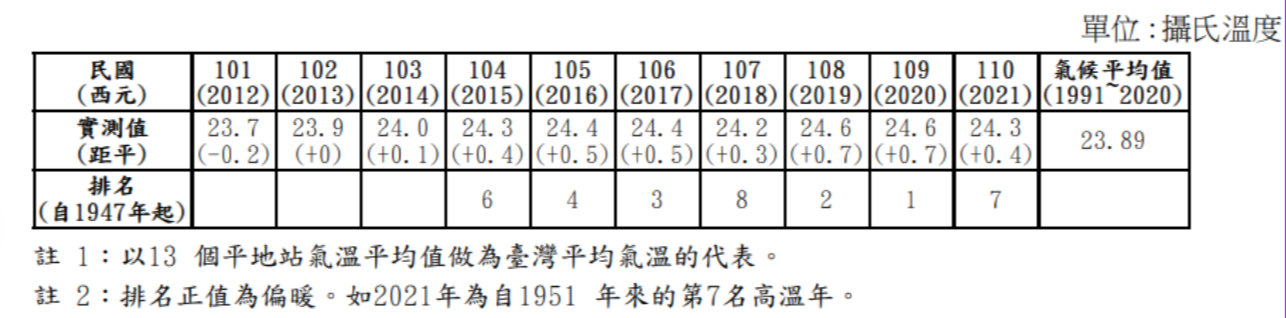
\includegraphics[width=0.8\textwidth]{tem.png}
    \caption{歷年7月氣溫距平值比較}
    \end{figure}

       2021(反聖嬰年)的黑潮強度減弱可能因赤道東風減弱導致海流變弱，
    而海峽因深度淺容易因大陸或海流影響溫度，因此黑潮減弱也讓海峽降溫。
    2016(聖嬰年)與反聖嬰年相反。
    在氣溫方面聖嬰年各地的溫度明顯較平均高出許多，
    而反聖嬰雖也升溫但整體升溫幅度並不高。年平均溫則較低。
\section{結論}
聖嬰現象對於台灣 7 月海域環境有顯著影響。
在聖嬰年，因大氣環流改變導致副熱帶高壓增強，台灣海峽呈現顯著的偏暖。
大尺度洋流調整促使黑潮強度在夏季有所提升。
相較之下，反聖嬰年的影響則較為分散。雖維持聖嬰年較熱，
反聖嬰年較冷的規律但藉由氣候數據還是可以發現每一年的氣溫都在增加，
可能受氣候變遷影響，
全球暖化的影響還是很劇烈，
{\titlespacing*{\section}{0pt}{1.5ex plus .1ex minus .2ex}{1pc}
\section{參考文獻}
\href{https://coastwatch.pfeg.noaa.gov}{NOAA SST Data}\\
\href{https://weilinlai719.github.io/earth-science-explore/}{探究website}\\
\href{https://www.cwa.gov.tw/Data/climate/Watch/twn/twn-monitor_2021-6.pdf}{CWA\ 2021年7月氣象監測報告}\\
\href{https://www.cwa.gov.tw/Data/climate/Watch/twn/twn-monitor_2016-6.pdf}{CWA\ 2016年7月氣象監測報告}
}
\end{document}